\section{Creating the documentation}

\subsection{Collaboration and hosting}

Before scaffolding the actual project or picking tools that might help me putting the documentation together, I thought about where to host and how to enable collaborative content editing. The obvious choice for my purposes was \textit{GitHub}, as it solves numerous problems in an elegant and user-friendly way.

\begin{description}

	\item[Hosting]\hfill

	\textit{GitHub} provides a feature called \textit{GitHub Pages}. With the help of a specific \textit{Git} branch (\enquote{gh-pages}), all files on this branch (from the latest revision) can be accessed via \ac{HTTP} on port 80. This means that static \ac{HTML} files are served as websites to any browser. The service is free of charge, is based on a reliable server infrastructure and leverages \textit{GitHub's} \ac{CDN} for improved response times. Updating the content is as easy as committing changes to the \textit{gh-pages} branch and pushing them to the remote repository.

	By default, the website's address is \texttt{http(s)://\allowbreak\textbf{user-name}.github.io/\allowbreak\textbf{project-name}}. But \textit{GitHub} allows advanced \ac{DNS} settings, enabling the repository maintainer to point custom domains to the project page.

	\item[Collaboration]\hfill

	Each project has an issue tracker that allows \textit{GitHub} users to notify the repository maintainer about problems he discovered. These issues are public and everybody is free to join the discussion to propose solutions or suggestions.

	Taking this one step further, users can enrich issues by adding code (or textual content) that attempts to solve the problems they were facing. This procedure is then called a \textit{pull-request}. For the repository maintainer, applying the provided patches to the project is as easy as pushing a single button to confirm.

	To simplify the audition process of \textit{pull-requests} it is possible to integrate third-party \ac{CI} services that automatically compile and test proposed changes and then add the their results and logs to the issue discussion.

	\item[Content editor]\hfill

	Every directory and file of a repository that is hosted on \textit{GitHub} can be browsed on their website. In addition to that, files can also be edited with an online text editor which allows to quickly update content without cloning the repository. This is especially useful for text-based projects like documentations because it is not necessary to compile or test the project before submitting a patch.

	Another positive side effect of this approach, is that a user's edits automatically result in \textit{pull-request} which can then be easily audited and approved as described earlier.

	\item[Popularity]\hfill

	\textit{GitHub} is incredibly well-known and established among developers. Users tend to know the described collaboration workflows which lowers the barrier to actually bring oneself to participating.

\end{description}

\subsection{Static page generator}

Although the goal of the documentation is to only consist of static \ac{HTML} files, I intended to integrate a static page generator in order to optimize the development process. This leads to a build step, necessary to compile the source code to basic \ac{HTML} files before committing to \textit{gh-pages}. But that's a low price to pay, considering the indispensable advantages of this approach.

\begin{description}

	\item[Templating]\hfill

	With a static site generator it is possible to split a document into several files which may then be included as desired. This is especially useful to avoid code duplication considering that certain elements like a page header or footer have to be included into every page. It does also allow to split each section of a long article into separate files which makes it easier to find one's way around when editing content.

	\item[Dialects]\hfill

	It is possible to process languages that could not be interpreted by a browser. E.g. converting \textit{CoffeeScript} to \textit{JavaScript}, \ac{SASS} to \ac{CSS} or \textit{Markdown} to \ac{HTML}.

	\item[Linting]\hfill

	To enforce best practices linting tools can be integrated into the build process that perform desired validations.

	\item[Custom tasks]\hfill

	An important requirement for the means of the documentation is the integration of custom build steps. They offer great flexibility and room for improvements. This way it is possible, for instance, to extract file information like the last time of an edit and inject them into the document, rather than maintaining this information manually. Or to apply syntax highlighting of code snippets at build time instead of relying on client sided code to perform such an optimization.

	\item[Post processing]\hfill

	In the last step of the build process it is now possible to apply minification tools to the \ac{HTML}, \ac{CSS} and \textit{JavaScript} sources. This file sizes are reduced significantly, improving the time it takes to load a page even further.

\end{description}

I originally started with a static page generator, called \textit{Roots}, that promised to solve most of these problems out of the box. It also integrates \textit{Markdown} processing which I intended to use to format textual content, because it is easier to maintain than \ac{HTML} code. But I realized rather quickly that such a tool is too specific and limiting for my purposes (especially regarding the custom build steps). Also \textit{Markdown} emerged to not fit in, as it didn't allow me to specify \ac{HTML} classes which would have been necessary to highlight certain paragraphs. My intention to create central sitemap, resource links and abbreviation indexes were also at risk as they could only be used with \textit{Markdown} by creating custom extensions. This cluttered up the documents and was in no way better to maintain than a more versatile \ac{HTML} templating system.

As a consequence of of these circumstances I migrated to \textit{Gulp}. \textit{Gulp} is, broadly spoken, a \textit{JavaScript} build tool for front-end development. The tool is famous for its simplicity and flexibility, but its greatest strength is the community around it that created thousands of plugins for every imaginable use case. Setting it up and getting the basics working to a similar range of functions like \textit{Roots} provides them was initially much more challenging. But in the long run I benefited from its flexibility as I was not forced to make a single compromise in this context.

Instead of \textit{Markdown} I switched to an \ac{HTML} templating system called \textit{Nunjucks}. It allowed me to split up my files and include them as necessary. To organize textual content as clearly as possible from the overall \ac{HTML} structure I was able to separate these concerns so much that content files only consist of headline, paragraph and image tags to then be included into the page, keeping them maintain- and readable.

To create \ac{CSS} assets I chose to integrate the \ac{SASS} preprocessor into the build chain as I made the experience in previous projects that it simplifies development tremendously. Also, I found myself writing very little \textit{JavaScript} code, so I kept that as simple as possible, not including any preprocessors or other additional tools except for \textit{jQuery}.

\subsection{Implementation}

\begin{description}

	\item[Content]\hfill

	The documentation as a whole is subdivided in numerous chapters which are each represented by a respective \ac{HTML} page. A table of contents is located on the root page offering to jump right into a topic of choice.

	\begin{enumerate}

		\item Introduction

		\item About this documentation

		An explanation of page features, but also a call to not shy away from contributing

		\item Prerequisites

		\item Build tool

		Comparison of \textit{Gradle} and \ac{SBT}, leaving room to add \textit{Gradle} documentation in the future

		\begin{enumerate}

			\item \ac{SBT}

		\end{enumerate}

		\item Project setup

		\item Editors and \acp{IDE}

		\begin{enumerate}

			\item \textit{IntelliJ IDEA}

			\item \textit{Android Studio}

		\end{enumerate}

		\item Working with the command line

		\item Dependencies

		\item \textit{ProGuard}

		\begin{enumerate}

			\item Cache

		\end{enumerate}

		\item \textit{Typed Resources (TR)}

		\item \textit{Parcelable}

		\item Testing

		\begin{enumerate}

			\item \textit{Robolectric}

		\end{enumerate}

		\item Library projects

		\item Publishing

	\end{enumerate}

	Besides these content chapters, there is a handful of additional pages that aim to help interpreting the documentation or to solve problems of which I took notice through the interviews.

	\begin{itemize}

		\item Fork me on \textit{GitHub}

		A typical catch phrase to point to a project's \textit{GitHub} repository. Clicking this link on the documentation website forwards the user directly to the respective \textit{GitHub} page.

		\item Getting help

		A list of development communities and resources that the reader should consider to consult when he gets stuck with \textit{Scala on Android}.

		\item Sources

		A large index of noteworthy websites (along with a content description) that contain information which might be relevant to further educate about a certain topic.

		\item Software

		A list of the software that was used to create the examples in the documentation. It also contains the particular version of the software as well as a download link.

		\item Abbreviations

		An abbreviation index.

	\end{itemize}

	\item[Responsive design]\hfill

	\begin{figure}[ht]
		\makebox[\textwidth][c]{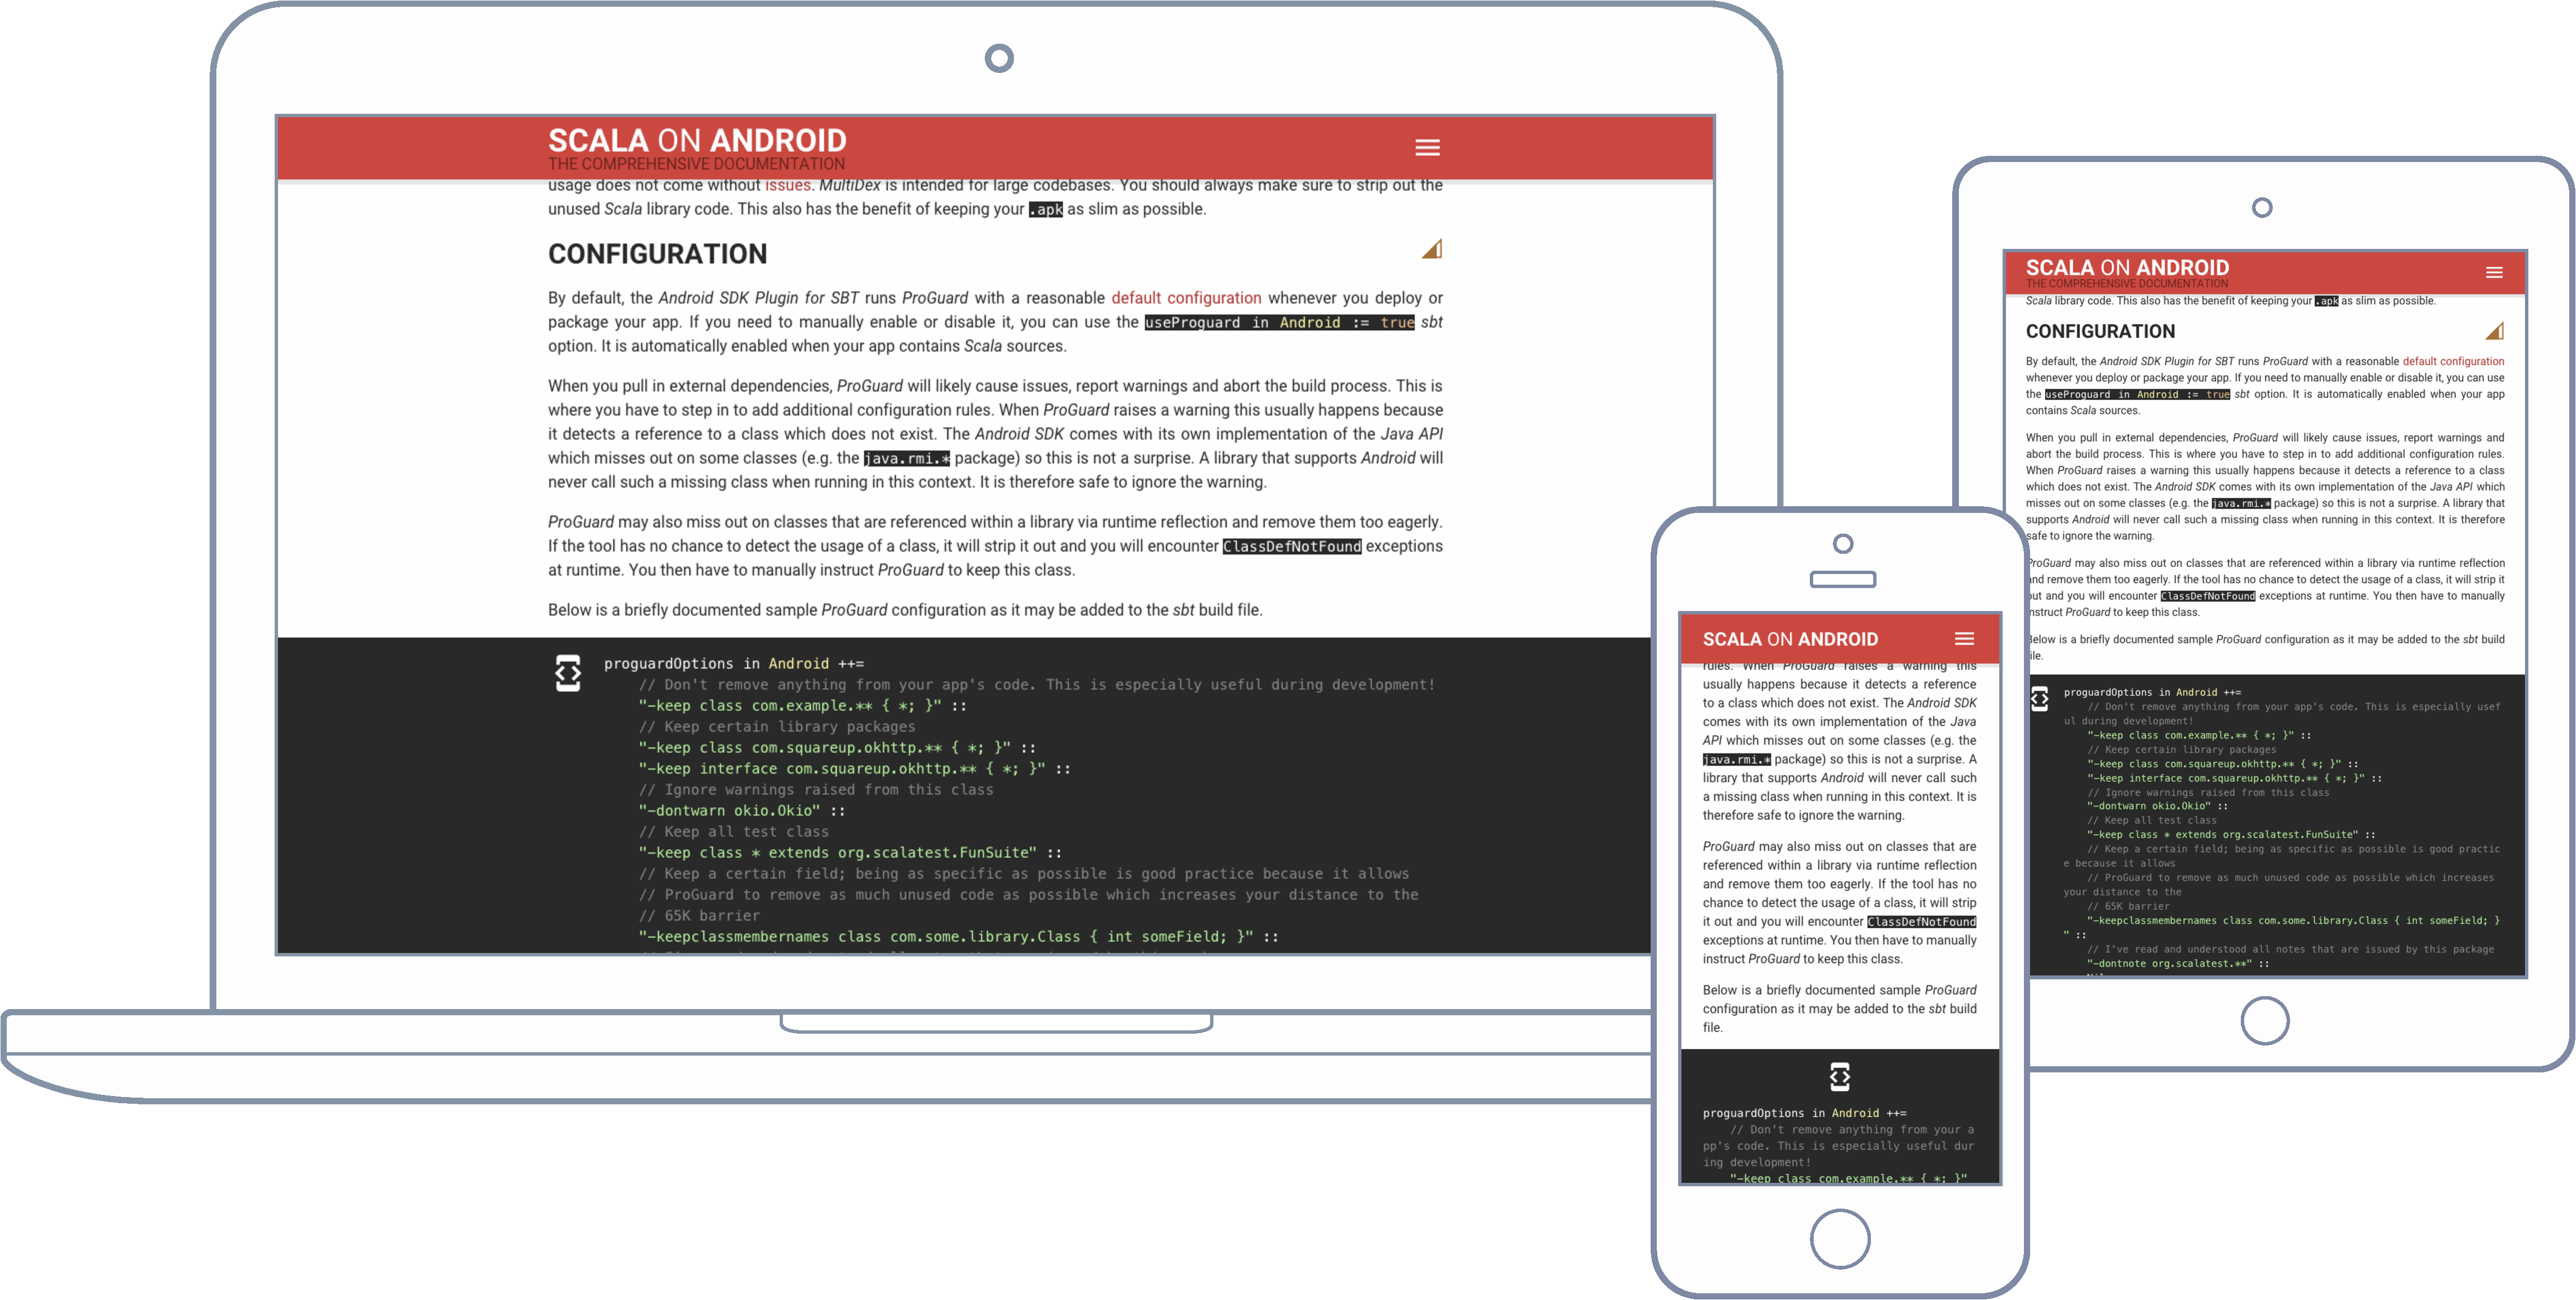
\includegraphics[width=1.5\textwidth]{asset/responsive-design.pdf}}
		\caption{Side by side comparison of the documentation website on common screen sizes}
		\label{responsive-design}
	\end{figure}

	Through \ac{CSS} \textit{Media Queries} the page automatically adjusts its properties in such way a that a pleasant reading experiences on all screen sizes and densities can always be guaranteed. Included graphics and icons are, wherever possible, delivered as \ac{SVG} assets. Furthermore, the page does refrain from using mouse hover events for crucial interaction since these would be inaccessible for mobile visitors with touchscreens (see figure \ref{responsive-design}).

	\item[Navigation]\hfill

	On the end of each chapter the user has the possibility to advance to the next topic to provide a natural reading flow (see figure \ref{story-telling}).

	Attached to the sticky header, bar there is also a navigation hidden behind the \textit{hamburger} icon that enables the user to jump to an arbitrary chapter (see figure \ref{navigation}).

	\begin{figure}[ht]
		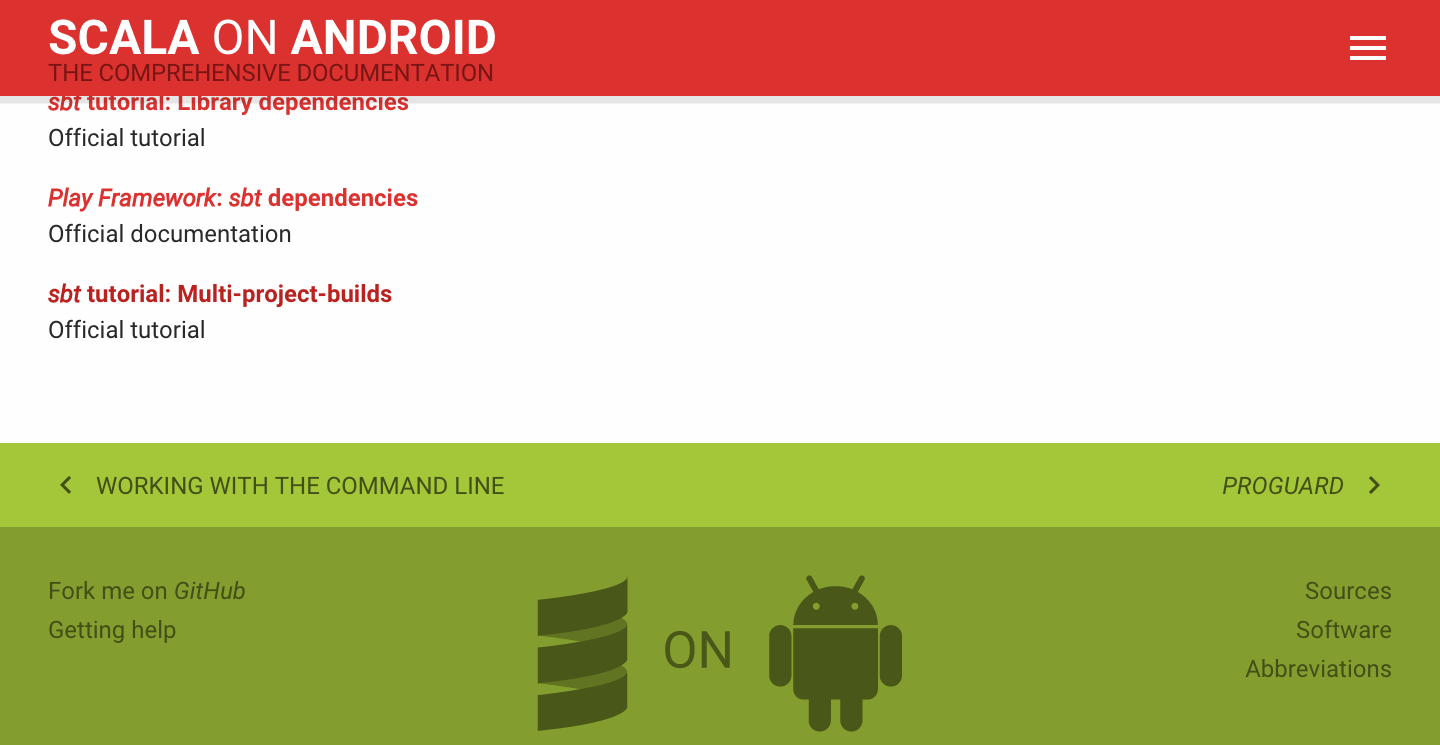
\includegraphics[width=\textwidth]{asset/story-telling.png}
		\caption{Footer navigation that contains a link to the previous and next chapter}
		\label{story-telling}
	\end{figure}

	\begin{figure}[ht]
		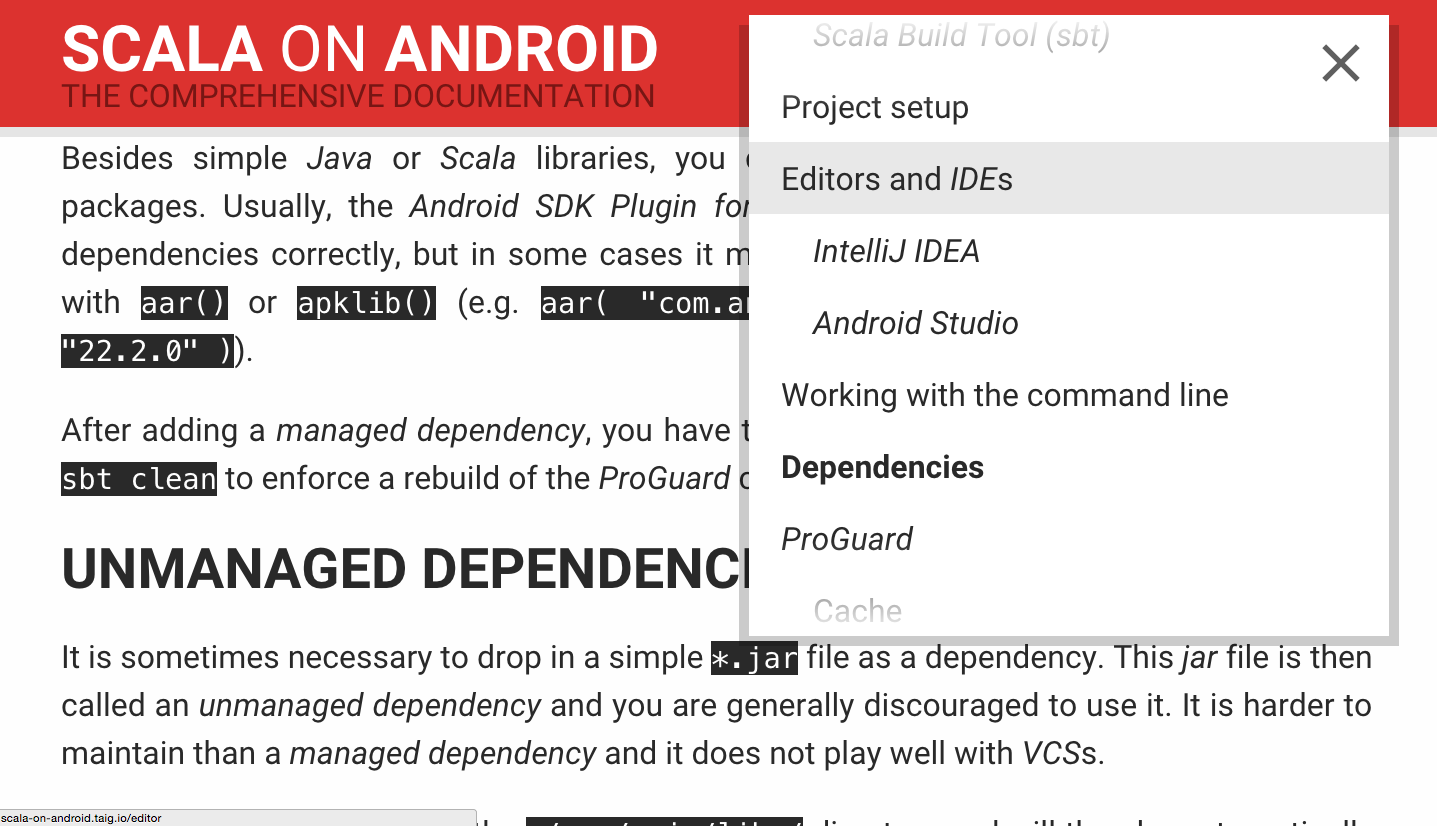
\includegraphics[width=\textwidth]{asset/navigation.png}
		\caption{Main navigation, attached to the sticky header}
		\label{navigation}
	\end{figure}

	\item[\textit{Metabox}]\hfill

	Next to each paragraph, there is a signal reception icon with the purpose to indicate information reliability. The ranking ranges from \textit{Fragile}, to \textit{Moderate} through to \textit{Sustainable} and is a representation of my personal impressions which I gathered while working with \textit{Scala on Android} or researched the particular topic (see figure \ref{reception-icons}).

	\begin{figure}[ht]
		\center
		
\includegraphics[width=6cm]{asset/reception-icons.png}
		\caption{Signal reception icons to indicate information reliability. \textit{Fragile} (left, red) and \textit{Moderate} (middle, orange), \textit{Sustainable} (right, green).}
		\label{reception-icons}
	\end{figure}

	Clicking on one of these signal icons leads to a \textit{Metabox} showing up. It contains an additional textual description of the information reliability, but also the date when the paragraph has been edited lately, enabling the reader to interpret the ranking in this context (see figure \ref{metabox}).

	\begin{figure}[ht]
		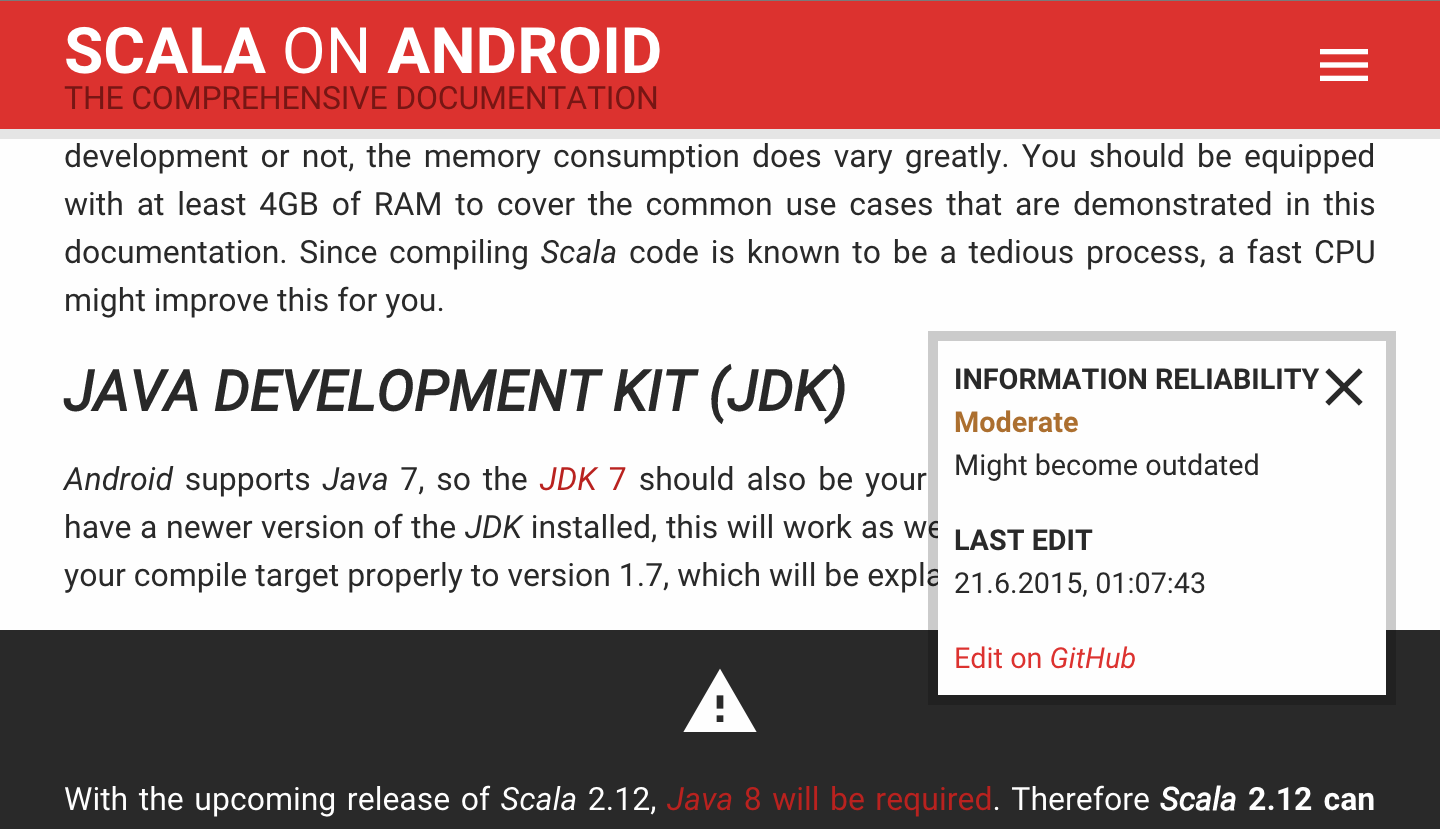
\includegraphics[width=\textwidth]{asset/metabox.png}
		\caption{A \textit{Metabox} that shows a \textit{Moderate} information reliability ranking.}
		\label{metabox}
	\end{figure}

	Another important element of the \textit{Metabox} is the \enquote{Edit on \textit{GitHub}} link. When clicked, a new tab with a text editor appears, encouraging the user to make changes. The text editor is part of the \textit{GitHub} website and once an edit has been made, a \textit{pull-request} is automatically created that I, as the the project maintainer, may then review and merge into the project to apply the patch. This approach provides a convenient collaboration workflow with the underlying \ac{VCS} and also reliefs me from the struggle to develop a similar feature.

	\item[Further reading]\hfill

	At the end of most chapters is the \enquote{Further reading} section. It contains links to articles and websites I used in order to put the provided information together. Since the overall structure of this section is the same on every page and numerous links were relevant to multiple chapters, I constructed a central sources index which contains entries that are shaped as shown below.

	\begin{code}{js}
'android':
{
	description: 'Official website',
	url: 'http://www.android.com/',
	title: 'Android'
},
'android-api-guides':
{
	description: 'Official documentation',
	url: 'https://developer.android.com/guide/index.html',
	title: 'Android API Guides'
},
...
	\end{code}

	With the help of the \ac{HTML} templating engine I could then create a function \texttt{section\_further\_reading()} that generates the section with minimal effort (see figure \ref{further-reading}).

	\begin{figure}[ht]
		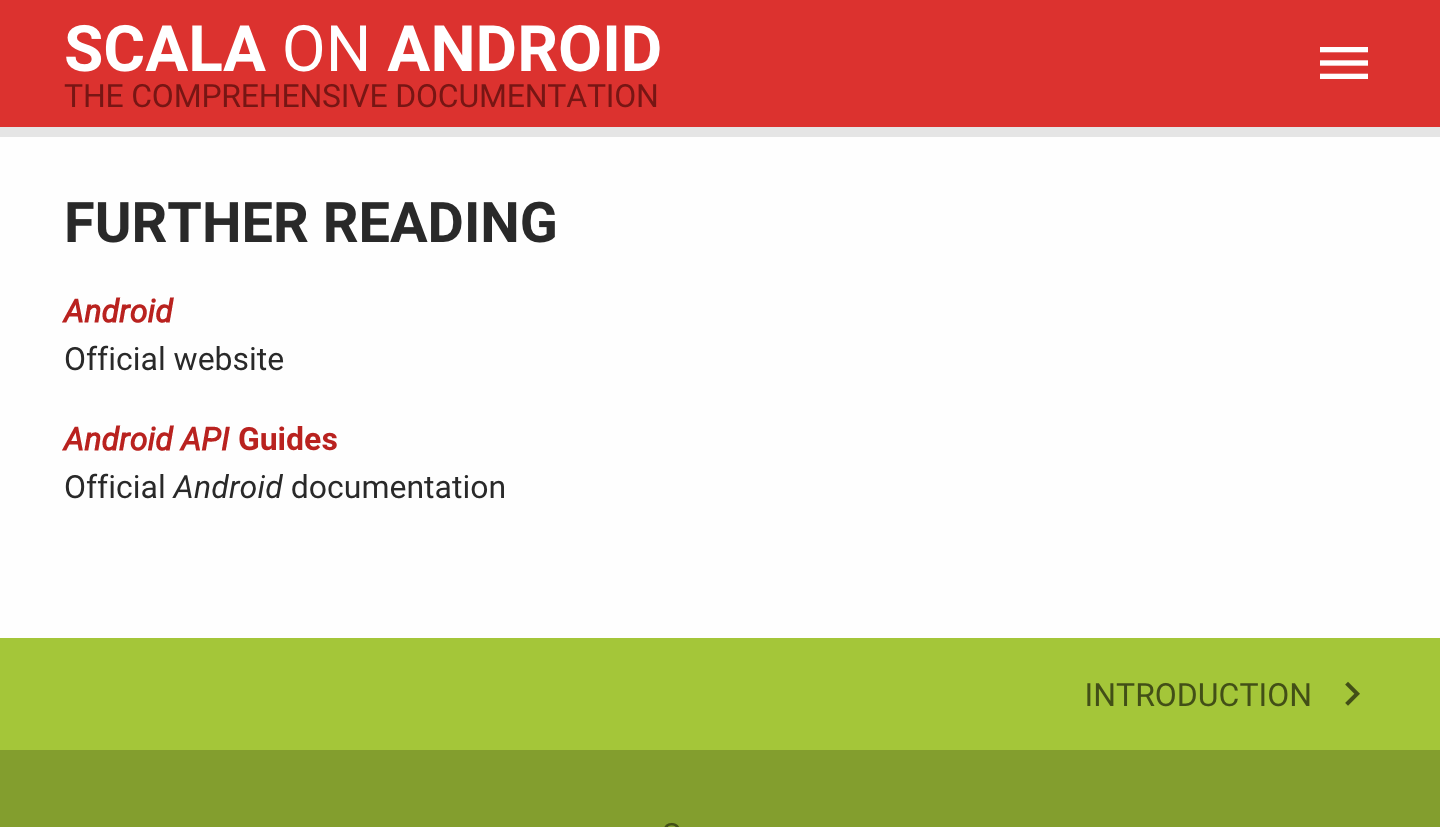
\includegraphics[width=\textwidth]{asset/further-reading.png}
		\caption{The further reading section at the end of a chapter.}
		\label{further-reading}
	\end{figure}

	\begin{code}{js}
section_further_reading( [ 'android', 'android-api-guides' ] );
	\end{code}

	Based on the index, the entire sources page is also generated automatically as part of the build process.

	\item[Abbreviations]\hfill

	Similar to the sources index, there is also a name index. I found myself repeating names of companies and technologies all over the place and intended to display them with an italic font. Additionally, in many cases, there are also common abbreviations for these names. To stop repeating myself and to be less prone to errors and inconsistencies, I introduced the names index.

	\begin{code}{js}
...
'robolectric': { name: 'Robolectric' },
'robotest': { name: 'RoboTest' },
'sbt':
{
	abbreviation: 'sbt',
	name: 'Scala Build Tool'
},
'sbt-plugin': { name: 'Android SDK Plugin for SBT' },
...
	\end{code}

	Allowing me to pull in names from the index into the template in this fashion:

	\begin{code}{js}
names.get( 'robolectric' ) // <em>Robolectric</em>
names.get( 'sbt' ) // <em>Scala Build Tool (sbt)</em>
names.abbr( 'sbt' ) // <abbr title="Scala Build Tool">sbt</abbr>
names.name( 'sbt' ) // <em>Scala Build Tool</em>
	\end{code}

	The major gain of this approach if the semantically valuable rendering of abbreviations with the \texttt{<abbr />} tag. If a reader is unfamiliar with an abbreviation, the title tooltip reveals the full meaning.

	Furthermore, I used all entries that contain a name and an abbreviation value to render the abbreviations page as part of the build process.

	\item[Highlighted paragraphs]\hfill

	A major reason that brought me to replace \textit{Markdown} with an \ac{HTML} templating system was the desire to highlight paragraphs that should stand out from the rest of the content. In \textit{Markdown} documents this could be achieved by embedding \ac{HTML} (which defeats the purpose of \textit{Markdown}) or, a surprisingly common practice, by abusing the blockquote syntax for this purpose. The templating engine allowed me to create a simple function that takes care of generating an appropriate markup, including an icon that illustrates why a paragraph was highlighted (see figures \ref{alert} and \ref{blockquote}).

	\begin{code}{html}

	<p>Lorem Ipsum</p>

	\end{code}

	This works for common text paragraphs, blockquotes and also code blocks without abusing \ac{HTML} elements in a context where they do not belong.

	\begin{figure}[ht]
		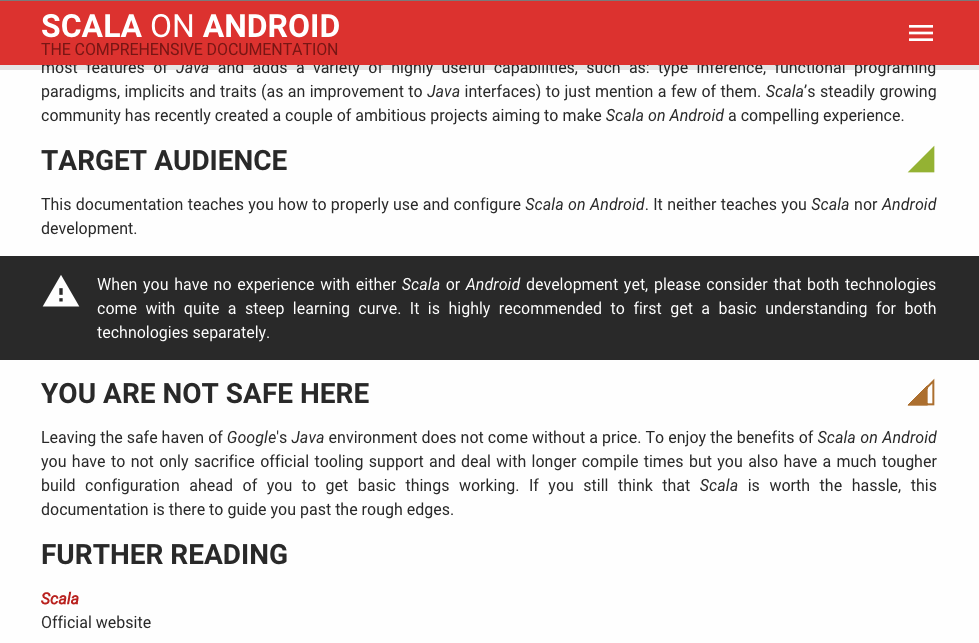
\includegraphics[width=\textwidth]{asset/alert.png}
		\caption{An example of a paragraph that is highlighted as an alert box to draw attention.}
		\label{alert}
	\end{figure}

	\begin{figure}[ht]
		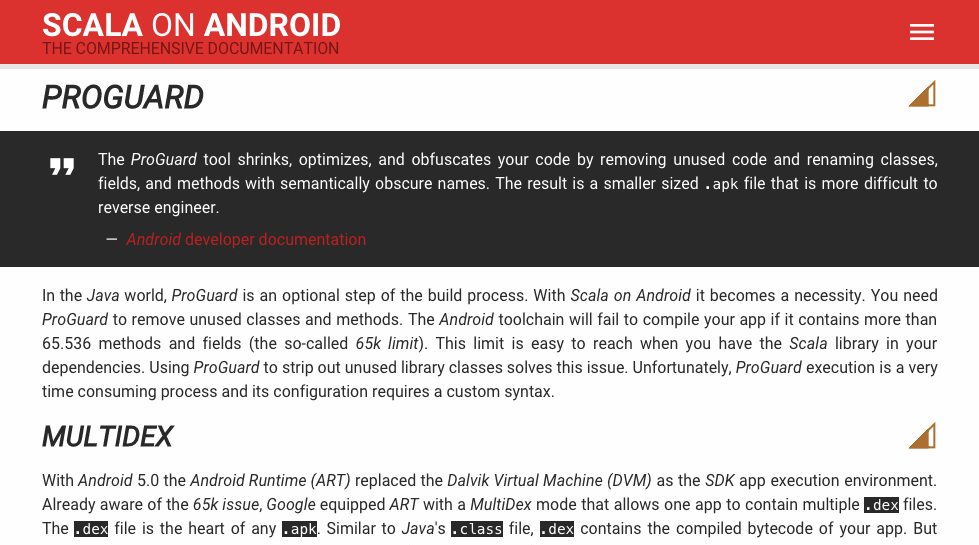
\includegraphics[width=\textwidth]{asset/blockquote.png}
		\caption{An example of a blockquote that is styled in the fashion of a highlighted paragraph.}
		\label{blockquote}
	\end{figure}

	\item[Syntax highlighting]\hfill

	In terms of styling, code blocks are basically just highlighted paragraphs (see figure \ref{syntax-highlighting}). But they were designed in such a way that the code may be placed in a separate file rather than inserting right into the \texttt{alert()} function body.

	\begin{code}{js}
// Render code file and apply Scala syntax highlighting
code( 'page/proguard/configuration.scala', 'scala' )
	\end{code}

	The actual highlighting of the program code is done by \textit{highlight.js} which is usually executed by the client. But since it was also possible to easily integrate it into the \textit{Gulp} build process I preferred to encode the syntax highlighting into the delivered \ac{HTML} documents. This way the client does not need to load the additional \textit{JavaScript} dependency and can also benefit from the feature when \textit{JavaScript} is not available.

	\begin{figure}[ht]
		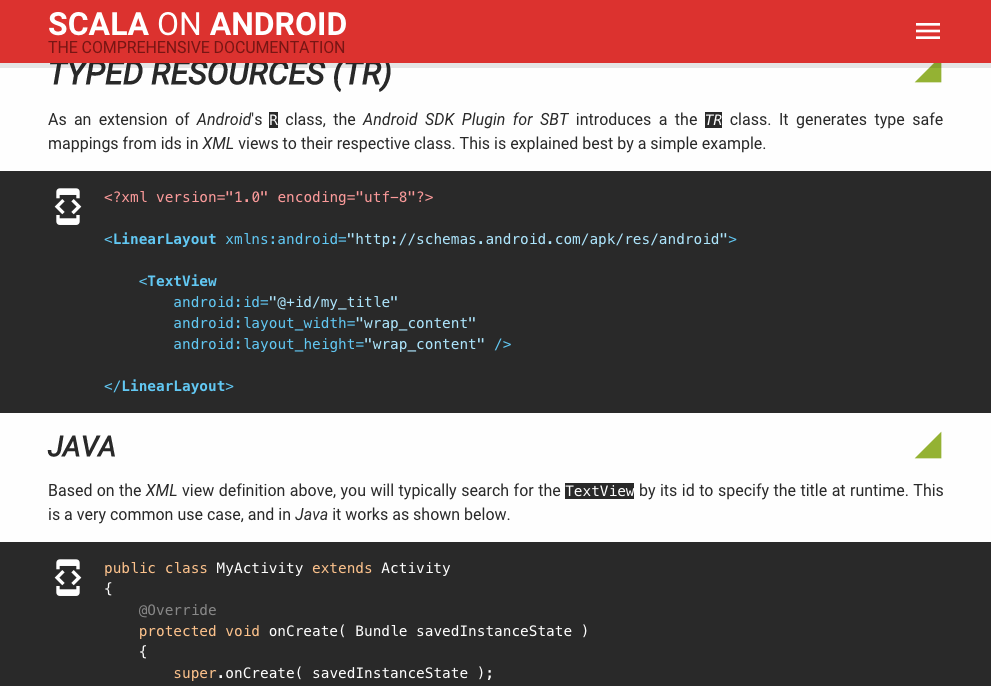
\includegraphics[width=\textwidth]{asset/syntax-highlighting.png}
		\caption{An example of code blocks that have syntax highlighting applied.}
		\label{syntax-highlighting}
	\end{figure}

	\item[\textit{Hello Scala}]\hfill

	Besides documenting how to set up and configure a \textit{Scala on Android} project I saw the need to create a comprehensive and executable project that implements the described practices. A lightweight configuration that is preconfigured with common dependencies (such as the \textit{Android} support libraries) and test cases. Just like the documentation, the \textit{Hello Scala} project is available on \textit{GitHub} and is intended to be cloned in order to have an up to date project template. The \textit{Scala on Android} documentation contains numerous references to its sister project, pointing out that there is a working example waiting to be explored (see figure \ref{hello-scala}).

	\begin{figure}[ht]
		\center
		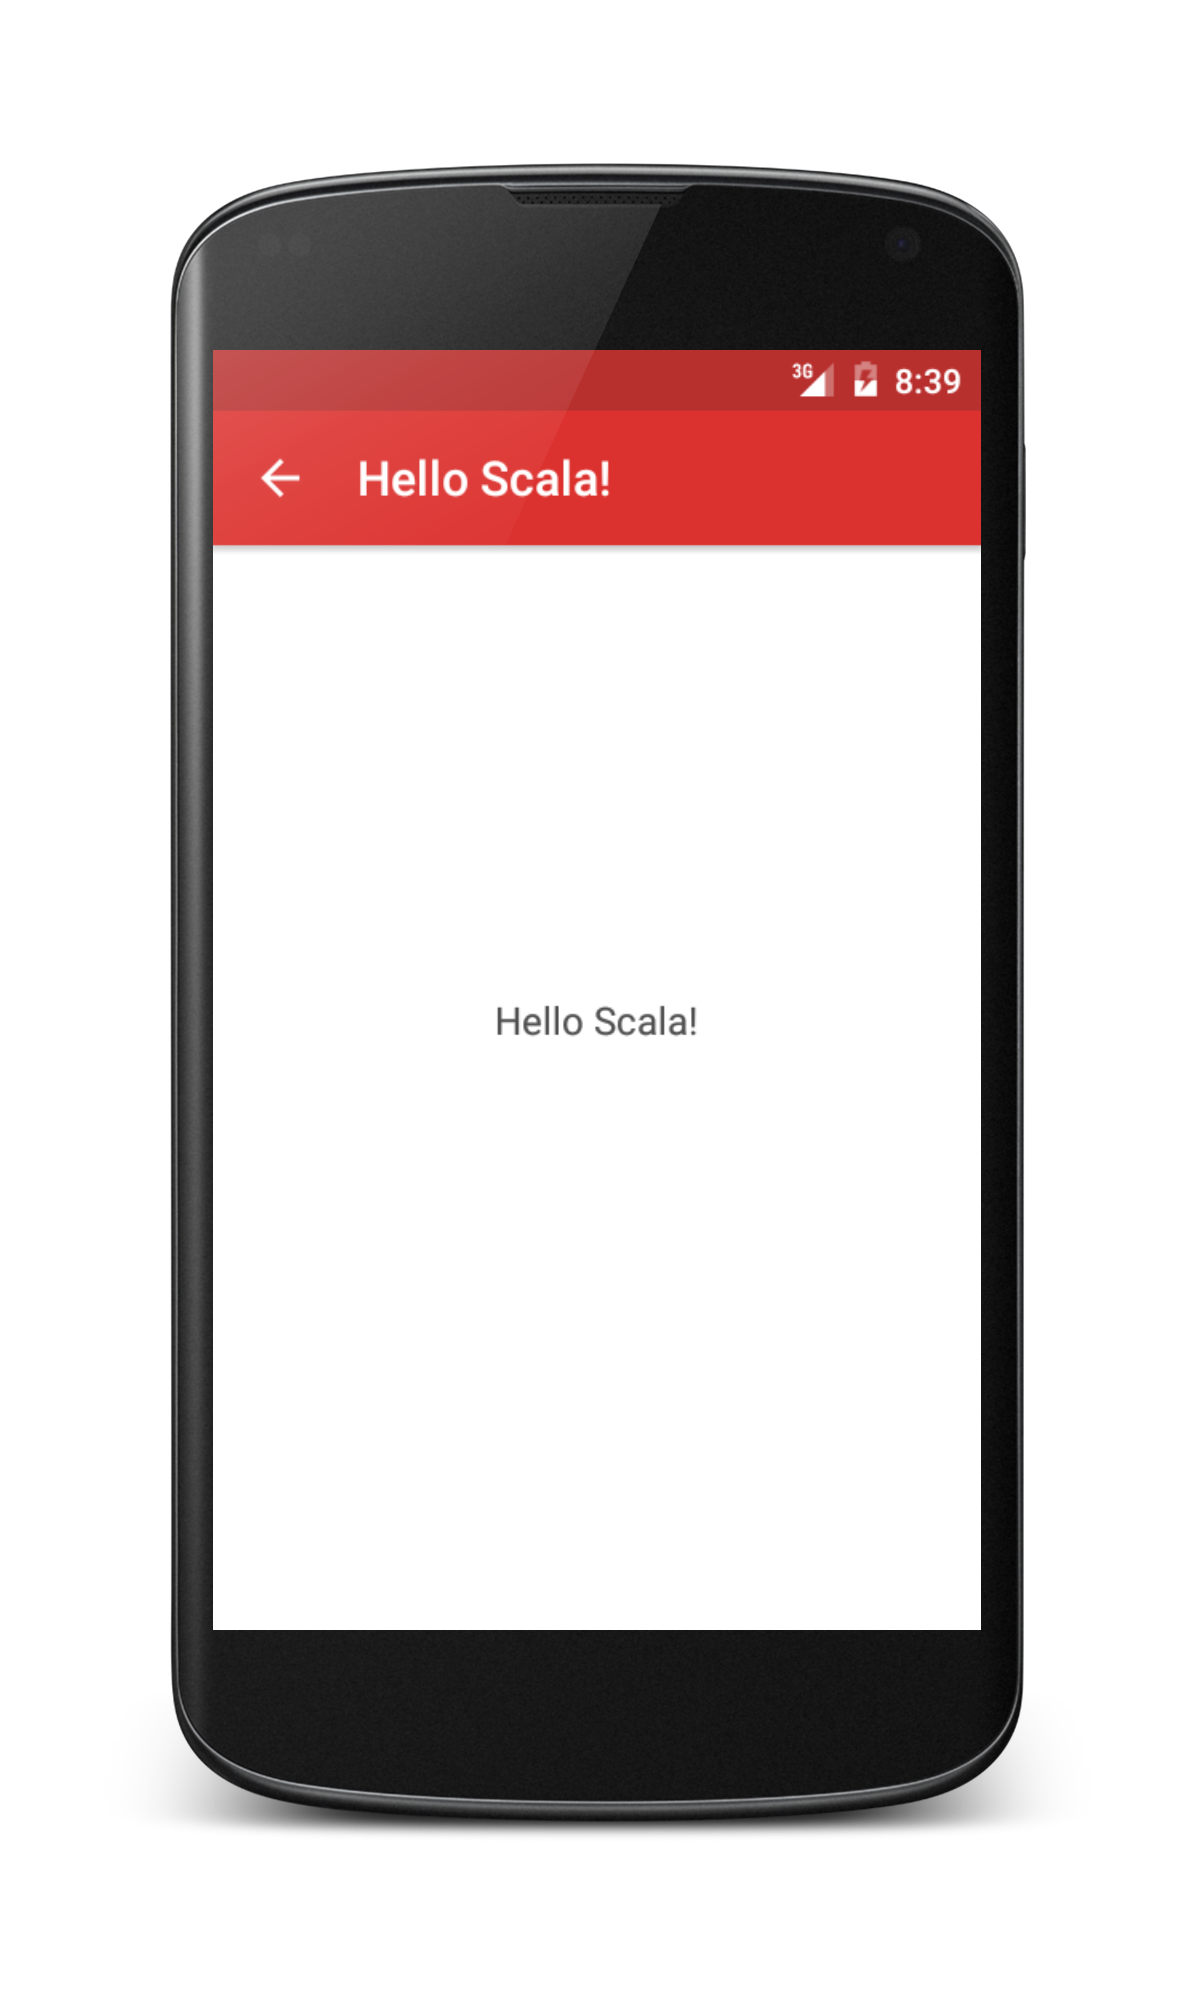
\includegraphics[width=0.6\textwidth]{asset/hello-scala.png}
		\caption{A screenshot of the \textit{Hello Scala} sample application}
		\label{hello-scala}
	\end{figure}

	\textit{HelloScala} aims to meet three important needs:

	\begin{description}

		\item[Curiosity]\hfill

		Newcomers should be able to clone and get it running on their device with minimal effort. Hoping a demonstrating of how easy a \textit{Scala on Android} set up can be encourages the visitor to give \textit{Scala on Android} a serious try.

		\item[Documentation]\hfill

		As it implements the best practices advertised in the documentation it serves as a functional showcase and learning resource.

		\item[Scaffolding]\hfill

		Rather than starting a new project from scratch, it should be a considerable alternative to clone the \textit{HelloScala} project as the foundation. It features a sophisticated \ac{SBT} configuration that can easily be trimmed down to specific needs rather than gathering up necessary configuration values from the web.

	\end{description}

\end{description}